\documentclass[8pt]{beamer}
\usepackage{verbatim}
\begin{document}
\title{TIAM+}
\subtitle{extending the Tool for Integrative Analysis of Motility\\ https://github.com/r-medina/TIAM-}
\author{Ricardo Medina}
\date{\today}

\frame{\titlepage}

\begin{frame}
  \frametitle{Task}
  \begin{figure}[H]\centering
    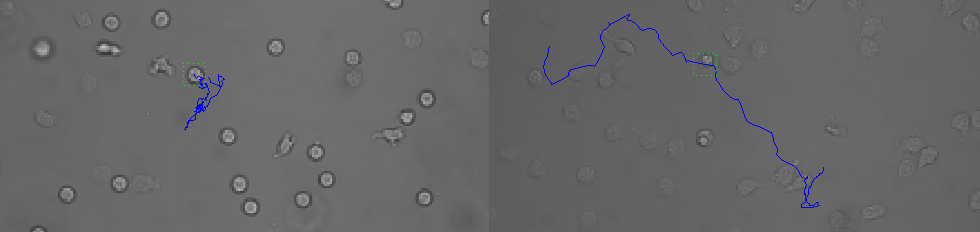
\includegraphics[width=.8\textwidth]{../fig/two_classes.png}
  \end{figure}
  Using data from Vivek Mayya and Willie Neiswanger's TIAM tool, which
  performs detection and tracking of cells from multi-channel time
  lapse microscopy videos, build an algorithm that will classify track
  segments. Two initial decisions:
  \begin{itemize}
  \item 2 classes
  \item $\therefore$ supervised
  \end{itemize}
  Goals:
  \begin{itemize}
  \item [$\checkmark$] collect supervised data
    \begin{itemize}
    \item Vivek used GUI Ricardo Medina developed to label each
      position of 126 cell tracks with IRM channel data as being in
      one of the two classes
    \end{itemize}
  \item [$\checkmark$] engineer/discover useful features for trajectory
    classification
  \item [$\checkmark$] find a supervised machine learning model that will work for
    the task at hand \emph{and} that will properly segment the cell tracks
  \item [?] develop an unsupervised generative model (HMM) with the help of Sakellarious Zairis and Jan-Willem van de Meent
  \end{itemize}
\end{frame}

\begin{frame}
  \frametitle{Supervised Histograms}
  \begin{figure}[H]\centering
    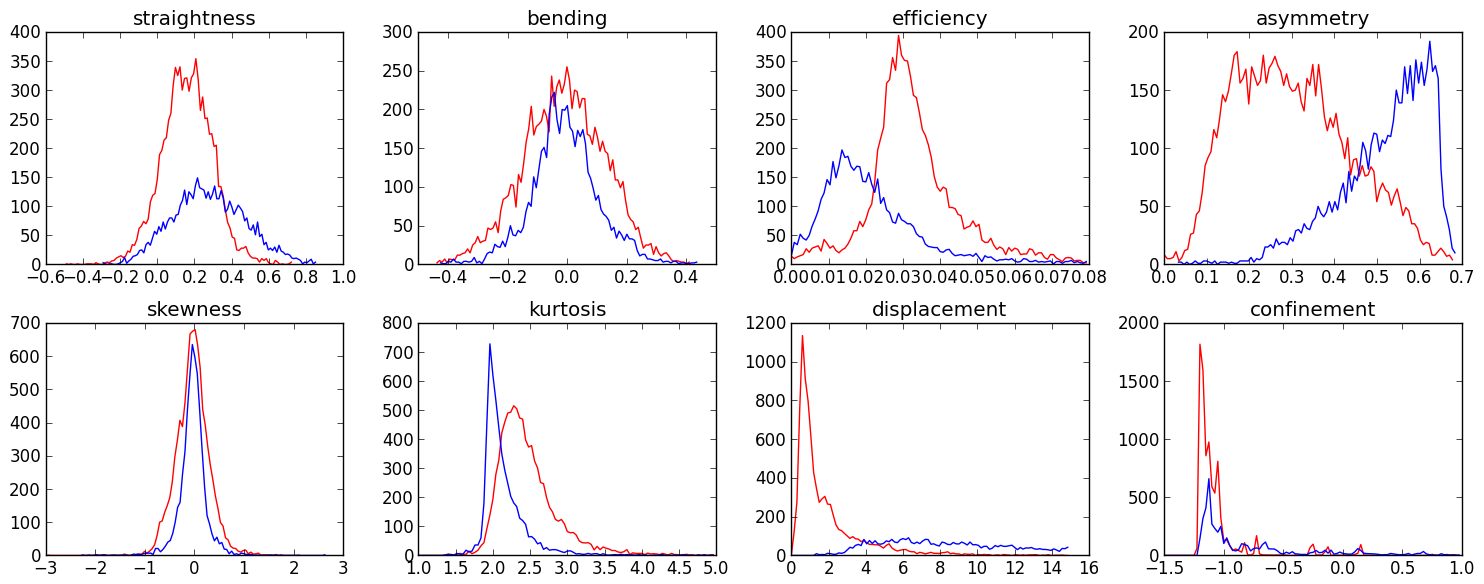
\includegraphics[width=\textwidth]{../../out/supervised_hist.png}
  \end{figure}
  \bigskip {\small \colorbox{red}{``Confined''} 
    \colorbox{blue}{``Not Confined''}}  
\end{frame}

\begin{frame}
  \frametitle{SVM Performance}
  Running the classifier on all data for which we have supervised labels (110 full
  trajectories with IRM channel data) gives the following result:
  \center{\begin{tabular}{r c|c l}
    true unconfined & 5048 & 454 & false confined \\
    \hline
    false unconfined & 487 & 8714 & true confined \\
  \end{tabular}}
  \begin{itemize}
  \item sensitivity: 0.917
  \item specificity: 0.947
  \item accuracy: 0.936
  \end{itemize}
  Woo!
\end{frame}

\begin{frame}
  \frametitle{SVM Histograms}
  \begin{figure}[H]\centering
    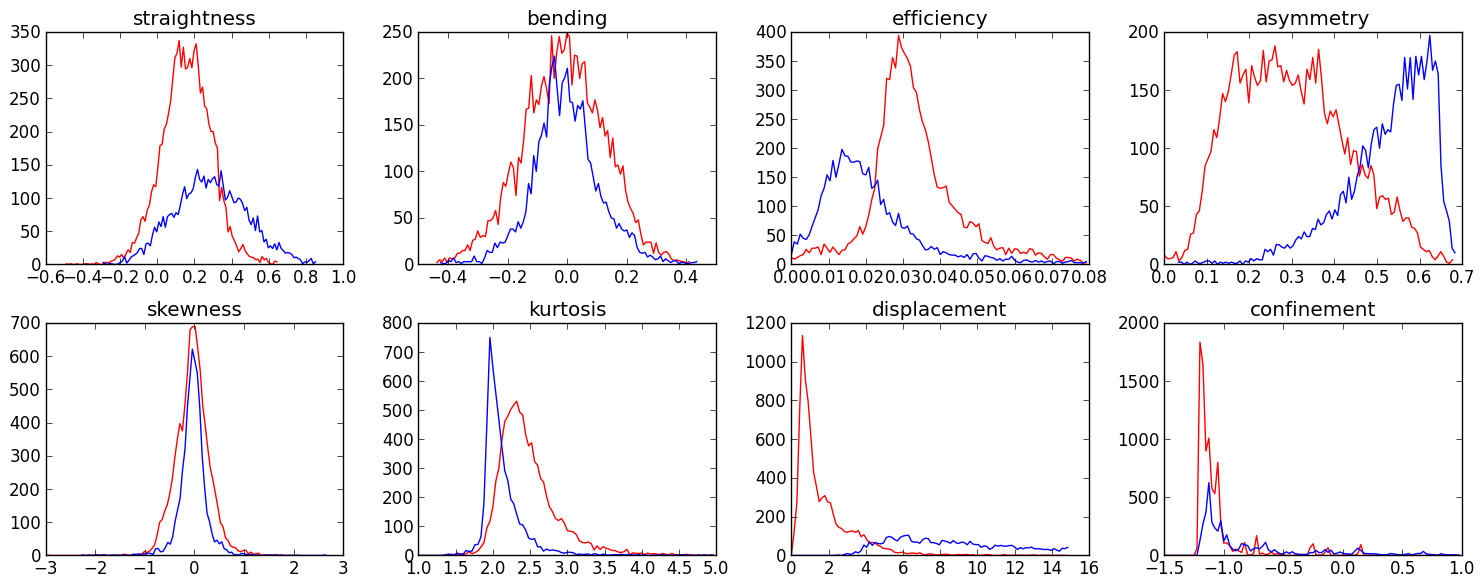
\includegraphics[width=\textwidth]{../../out/svm_hist.png}
  \end{figure}
  \bigskip {\small \colorbox{red}{``Confined''} 
    \colorbox{blue}{``Not Confined''}}
  
\end{frame}




\end{document}



%%% Local Variables: 
%%% mode: latex
%%% TeX-master: t
%%% End: 
